\section{Recognition Strategies}
\label{sec:background:recognition_strategies}

The \gls{icdar} robust reading competitions \citep{Lucas:2003iw, Lucas:2005bq, Shahab:2011hq} broke down the issue of text extraction into two sub-problems: text locating and character recognition. Most of the literature discussed in Section~\ref{sec:background:detection_strategies} focused within the text locating sub-problems; there were no expressions of interest in character recognition in \gls{icdar} 2003 and 2005 and only three in 2011 (the top system \citep{Liu:2005uw} scoring a correct recognition rate of 41.2\%).

It has been widely demonstrated that off-the-shelf commercial and open source OCR packages \todo{cite and find which ones were used} are able to correctly recognise text once the characters are extracted. Recent interest in developing novel general character recognition strategies has been rather stagnant, though there are exceptions for specific recognition cases.

\begin{figure}[h]
  \centering
  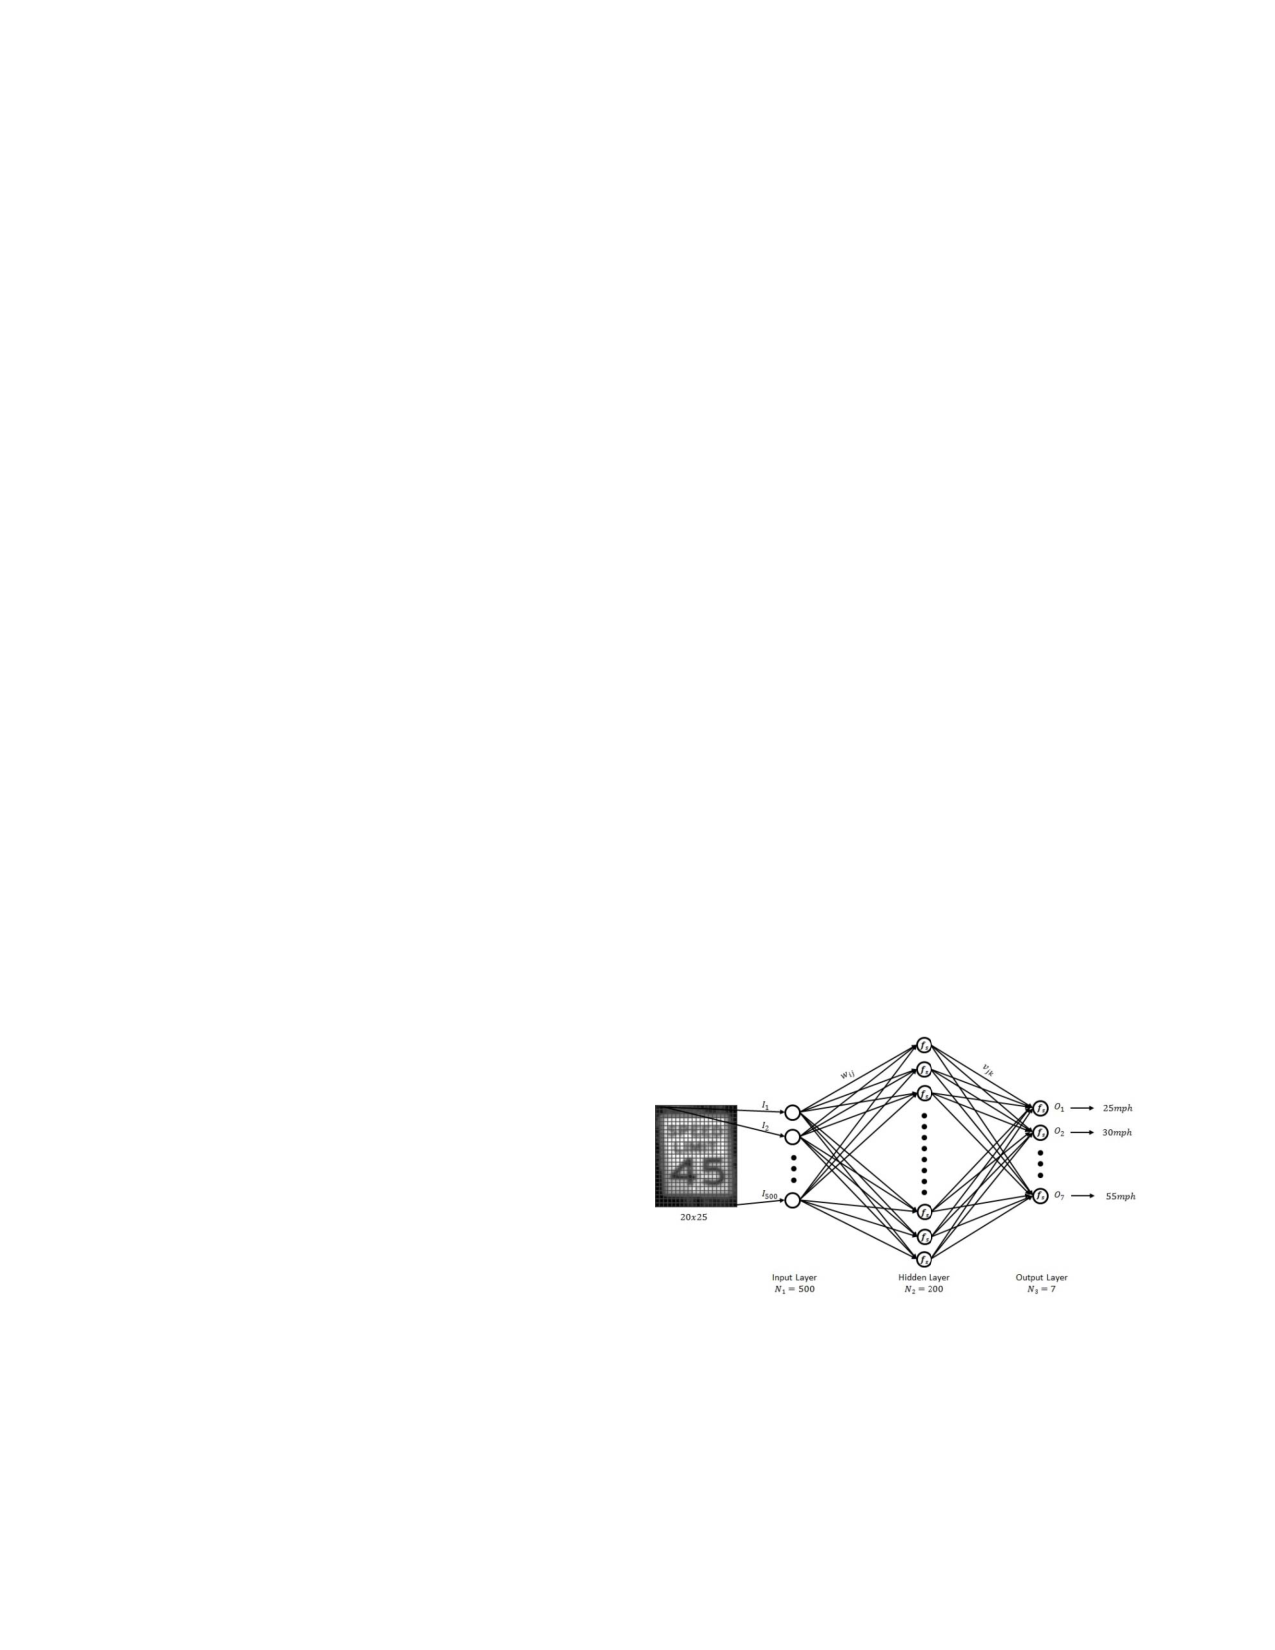
\includegraphics[width=\textwidth]{images/background/kundu2015_nn}
  \caption[A NN designed to recognised speed limit signs]{The artificial \glsx{mlp} \gls{nn} designed in \citet{Kundu:2015vq} to recognise US-style speed limit signs.}
  \label{fig:background:recognition:kundu2015_nn}
\end{figure}

A \citeyear{Kundu:2015vq} study into \glsplx{tsr} to detect US-style speed limit signs achieved recognition without the use of any OCR packages. In \citep{Kundu:2015vq}, \citeauthor{Kundu:2015vq} were able to extract a speed limit sign via the use of \glspl{mser} and template matching. The resulting detected signs were scaled to a grayscaled size of $20 \times 25$ pixels and fed into a \glsx{mlp} \gls{nn} of 200 neurons in the hidden layer. The output layer of the network consisted of seven nodes, each representing the seven kinds of speed limit signs in US cities (25, 30, 35, 40, 45, 50, and 55 miles per hour). This architecture is shown in Figure~\ref{fig:background:recognition:kundu2015_nn}. When trained with 13,289 images of text cases and 4,319 non-text cases, the results showed that their recognition classier was able to correctly recognise speed limit signs with an accuracy of 98.04\%.

Similar results were found in \todo{find other studies using NN in speed limits, like the one with x0 numbers}.

However, these networks are generally non-generalisable and only work in a limited context (i.e., by classifying speed limit signs of known outputs). In our context of \gls{rbn}, we have a known character output range of 36 possibilities (0--9 and A--Z) 

% Talk about BIB literature
% Talk about number plate literature
% Talk about speed sign NN literature